% -----------------------------------------------------------------
% Document class: Article
\documentclass[ a4paper, twoside, 11pt]{article}
\usepackage{../../macros-general}
\usepackage{../../macros-article}
% Number of the handout, quiz, exam, etc.
\newcommand{\numero}{02}
\setcounter{numero}{\numero}

% -----------------------------------------------------------------
\begin{document}
\allowdisplaybreaks

\begin{center}
\Large Modelos Estoc\'asticos (INDG-1008): Lecci\'on \numero \\[1ex]
\small \textbf{Semestre:} 2017-2018 T\'ermino I \qquad
\textbf{Instructor:} Luis I. Reyes Castro
\end{center}
\halfskip

\fbox{

\begin{minipage}[b][\height][t]{\textwidth}
\vspace{0.2 cm}

\begin{center}
\textbf{COMPROMISO DE HONOR}
\end{center}
\vspace{0.4 cm}

\scriptsize
{
Yo, \rule{60mm}{.1pt} al firmar este compromiso, reconozco que la presente evaluaci\'on est\'a dise\~nada para ser resuelta de manera individual, que puedo usar un l\'apiz o pluma y una calculadora cient\'ifica, \linebreak que solo puedo comunicarme con la persona responsable de la recepci\'on de la evaluaci\'on, y que cualquier instrumento de comunicaci\'on que hubiere tra\'ido debo apagarlo. Tambi\'en estoy conciente que no debo consultar libros, notas, \linebreak ni materiales did\'acticos adicionales a los que el instructor entregue durante la evaluaci\'on o autorice a utilizar. Finalmente, me comprometo a desarrollar y presentar mis respuestas de manera clara y ordenada. \\

Firmo al pie del presente compromiso como constancia de haberlo le\'ido y aceptado. 
\vspace{0.4 cm}

Firma: \rule{60mm}{.1pt} \qquad N\'umero de matr\'icula: \rule{40mm}{.1pt} \hspace{0.5cm} \\[-0.8ex]
}

\end{minipage}

}

\vspace{\baselineskip}



% -----------------------------------------------------------------
\begin{problem}
\textbf{[3 Puntos]} Una empresa est\'a tratando de decidir qu\'e hacer con el software que usa para su operaci\'on principal. Tal como se muestra en el siguiente \'arbol de decisi\'on, \linebreak la empresa puede desarrollar su propio software, comprarlo, o seguir utilizando el mismo que tiene actualmente. Determine la decisi\'on \'optima. 

\begin{figure}[htb]
\centering
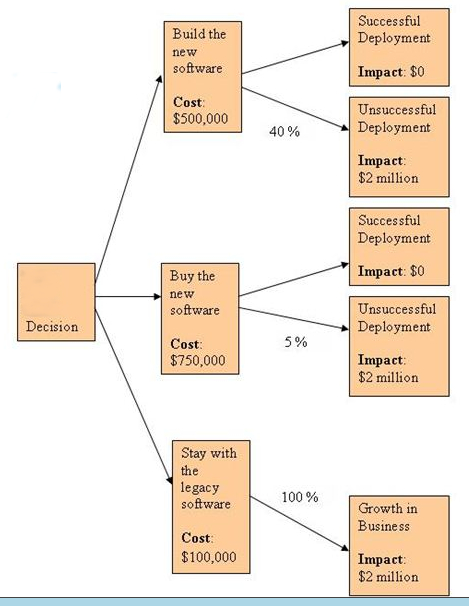
\includegraphics[width=0.5\textwidth]{problema_arbol-decision.jpg}
\end{figure}

\emph{Soluci\'on:} Analizamos el valor esperado de cada decisi\'on:
\begin{itemize}
\item Si la empresa desarrolla su propio software su costo es:
\begin{itemize}
\item \$500,000 con probabilidad del 60\%
\item \$2,500,000 con probabilidad del 40\%
\end{itemize}
Consecuentemente su costo esperado es de:
\[
(\$500,000)(0.6) + (\$2,500,000)(0.4) \; = \; \$1,300,000
\]
\item Si la empresa compra el software su costo es:
\begin{itemize}
\item \$750,000 con probabilidad del 95\%
\item \$2,750,000 con probabilidad del 5\%
\end{itemize}
Consecuentemente su costo esperado es de:
\[
(\$750,000)(0.95) + (\$2,750,000)(0.05) \; = \; \$850,000
\]
\item Si la empresa sigue utilizando el mismo software entonces su costo es de \$2,100,000 con probabilidad unitaria. Consecuentemente su costo esperado es el mismo.
\end{itemize}
En conclusi\'on, la decisi\'on \'optima es comprar el software.

\end{problem}
\vspace{\baselineskip}

% -----------------------------------------------------------------
\begin{problem}
\textbf{[3 Puntos]} Considere el siguiente modelo de litigio en cortes estadounidenses, el cual es basado en un modelo publicado en la p\'agina web \emph{Settlement Perspectives} del abogado John DeGroot en un art\'iculo titulado ``Decision Tree Analysis in Litigation: The Basics'' y publicado el 4 de enero del 2009. El modelo especifica un \'arbol de probabilidad que representa los diferentes escenarios de un litigio desde el punto de vista de la parte acusadora. Con esto en mente, calcule la ganancia esperada de la parte acusadora. 

\begin{figure}[H]
\centering
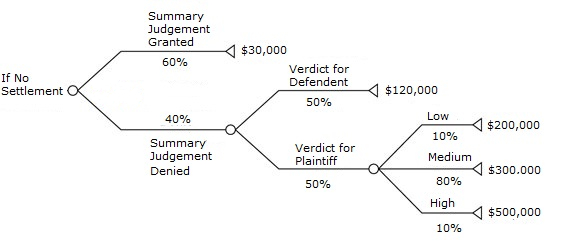
\includegraphics[width=0.9\textwidth]{problema_arbol-recompensas.jpg}
\end{figure}

\emph{Soluci\'on:} Procedemos por etapas: 
\begin{enumerate}
\item Evaluamos la utilidad del nodo `Veredict for Plaintiff': 
\[
(0.1)(\$200,000) + (0.8)(\$300,000) + (0.1)(\$500,000) \; = \; \$310,000
\]
\item Evaluamos la utilidad del nodo `Summary Judgement Denied': 
\[
(0.5)(\$120,000) + (0.5)(\$310,000) \; = \; \$215,000
\]
\item Evaluamos la utilidad del nodo `If No Settlement': 
\[
(0.6)(\$30,000) + (0.4)(\$215,000) \; = \; \$104,000
\]
\end{enumerate}
En conclusi\'on, la ganancia esperada de la parte acusadora es de \$104,000. 

\end{problem}
\vspace{\baselineskip}

% -----------------------------------------------------------------
\begin{problem}
Una empresa est\'a contemplando el lanzamiento de un nuevo producto. Si el producto tiene \'exito, lo cual se cree que ocurrir\'a con una probabilidad del 65\%, la empresa lograr\'a acumular alrededor de \$60,000 d\'olares en ganancias; en cambio, si el producto fracasa, la empresa perder\'a alrededor de \$40,000. Se sobre-entiende que la empresa tambi\'en puede optar por no lanzar el producto. Usted se dedica a organizar \emph{focus groups} para evaluar nuevos productos, los cuales predicen correctamente el \'exito o fracaso de un nuevo producto el 90\% de las veces. Actualmente, usted cobrar\'ia unos \$1,200 por evaluar el nuevo producto de la empresa antes mencionada. 

Con esto en mente, complete las siguientes actividades: 
\begin{itemize}
\item \textbf{[4 Puntos]} Suponiendo que usted le ofrece sus servicios al gerente de la empresa, modele el problema de decisi\'on del gerente como un \'arbol. 
\item \textbf{[4 Puntos]} Calcule la utilidad esperada de la empresa y describa la pol\'itica \'optima. 
\end{itemize}

\emph{Soluci\'on:} Definimos las siguientes variables aleatorias: 
\begin{itemize}
\item $X \in \{ 0, 1\}$ denota si el producto fracasa o es exitoso
\item $Y \in \{ 0, 1\}$ denota si el focus group predice \'exito o fracaso
\end{itemize}
Empezamos calculando las probabilidades posteriores:
\begin{align*}
\Pr(Y=1) \;
& = \; \Pr(X=1) \cdot \Pr(Y=1|X=1)
+ \Pr(X=0) \cdot \Pr(Y=1|X=0) \\
& = \; (0.65)(0.90) + (0.35)(0.10) \; = \; 0.62 \\
\Longrightarrow \; \Pr(Y=0) \; & = \; 0.38
\end{align*}
Luego calculamos las probabilidades priores condicionales en las posteriores: 
\begin{itemize}
\item Para el caso cuando el focus group predice \'exito, tenemos: 
\begin{align*}
\Pr( X=1 \mid Y=1 ) \;
& = \; \frac{ \Pr(X=1) \cdot \Pr( Y=1 \mid X=1 ) }{\Pr(Y=1)} \\[1ex]
& = \; \frac{ (0.65)(0.90) }{(0.62)} \; = \; 0.94 \\[1ex]
\Longrightarrow \; \Pr( X=0 \mid Y=1 ) \;
& = \; 0.06
\end{align*}
\item Para el caso cuando el focus group predice fracaso, tenemos: 
\begin{align*}
\Pr( X=1 \mid Y=0 ) \;
& = \; \frac{ \Pr(X=1) \cdot \Pr( Y=0 \mid X=1 ) }{\Pr(Y=0)} \\[1ex]
& = \; \frac{ (0.65)(0.10) }{(0.38)} \; = \; 0.17 \\[1ex]
\Longrightarrow \; \Pr( X=0 \mid Y=0 ) \;
& = \; 0.83
\end{align*}
\end{itemize}

Con todas las probabilidades calculadas podemos ahora construir el \'arbol de decisi\'on: 
\begin{itemize}

\item Decisi\'on: No contratar el focus group
\begin{itemize}
\item Decisi\'on: Lanzar el producto
\begin{itemize}
\item Escenario con probabilidad $\Pr(X=1) = 0.65$ : Producto es exitoso
\[
\text{Utilidad} \; = \; +\$60,000
\]
\item Escenario con probabilidad $\Pr(X=0) = 0.35$ : Producto fracasa
\[
\text{Utilidad} \; = \; -\$40,000
\]
\end{itemize}
\item Decisi\'on: No lanzar el producto
\[
\text{Utilidad} \; = \; \$0
\]
\end{itemize}

\item Decisi\'on: Contratar el focus group
\begin{itemize}

\item Escenario con probabilidad $\Pr(Y=1) = 0.62$ : Focus group predice \'exito
\begin{itemize}
\item Decisi\'on: Lanzar el producto
\begin{itemize}
\item Escenario con probabilidad $\Pr( X=1 \mid Y=1 ) = 0.94$ : Producto es exitoso
\[
\text{Utilidad} \; = \; +\$58,800
\]
\item Escenario con probabilidad $\Pr( X=0 \mid Y=1 ) = 0.06$ : Producto fracasa
\[
\text{Utilidad} \; = \; -\$41,200
\]
\end{itemize}
\item Decisi\'on: No lanzar el producto
\[
\text{Utilidad} \; = \; -\$1,200
\]
\end{itemize}

\item Escenario con probabilidad $\Pr(Y=0) = 0.38$ : Focus group predice fracaso.
\begin{itemize}
\item Decisi\'on: Lanzar el producto
\begin{itemize}
\item Escenario con probabilidad $\Pr( X=1 \mid Y=0 ) = 0.17$ : Producto es exitoso
\[
\text{Utilidad} \; = \; +\$58,800
\]
\item Escenario con probabilidad $\Pr( X=0 \mid Y=0 ) = 0.83$ : Producto fracasa
\[
\text{Utilidad} \; = \; -\$41,200
\]
\end{itemize}
\item Decisi\'on: No lanzar el producto
\[
\text{Utilidad} \; = \; -\$1,200
\]
\end{itemize}
\end{itemize}

\end{itemize}

Primera iteraci\'on de programaci\'on din\'amica: 
\begin{itemize}

\item Decisi\'on: No contratar el focus group
\begin{itemize}
\item Decisi\'on: Lanzar el producto
\[
\Exp(\text{Utilidad}) \; = \;
(0.65)(+\$60,000) + (0.35)(-\$40,000) \; = \; +\$25,000
\]
\item Decisi\'on: No lanzar el producto
\[
\text{Utilidad} \; = \; \$0
\]
\end{itemize}

\item Decisi\'on: Contratar el focus group
\begin{itemize}

\item Escenario con probabilidad $\Pr(Y=1) = 0.62$ : Focus group predice \'exito
\begin{itemize}
\item Decisi\'on: Lanzar el producto
\[
\Exp(\text{Utilidad}) \; = \;
(0.94)(+\$58,800) + (0.06)(-\$41,200) \; = \; +\$52,800
\]
\item Decisi\'on: No lanzar el producto
\[
\text{Utilidad} \; = \; -\$1,200
\]
\end{itemize}

\item Escenario con probabilidad $\Pr(Y=0) = 0.38$ : Focus group predice fracaso.
\begin{itemize}
\item Decisi\'on: Lanzar el producto
\[
\Exp(\text{Utilidad}) \; = \;
(0.17)(+\$58,800) + (0.83)(-\$41,200) \; = \; -\$24,200
\]
\item Decisi\'on: No lanzar el producto
\[
\text{Utilidad} \; = \; -\$1,200
\]
\end{itemize}
\end{itemize}

\end{itemize}

Segunda iteraci\'on de programaci\'on din\'amica: 
\begin{itemize}

\item Decisi\'on: No contratar el focus group y lanzar el producto
\[
\Exp(\text{Utilidad}) \; = \; +\$25,000
\]

\item Decisi\'on: Contratar el focus group
\begin{itemize}
\item Escenario con probabilidad $\Pr(Y=1) = 0.62$ : Focus group predice \'exito y se lanza el producto
\[
\Exp(\text{Utilidad}) \; = \; +\$52,800
\]
\item Escenario con probabilidad $\Pr(Y=0) = 0.38$ : Focus group predice fracaso y no se lanza el producto
\[
\Exp(
\text{Utilidad} \; = \; -\$1,200
\]
\end{itemize}

\end{itemize}

Tercera iteraci\'on de programaci\'on din\'amica: 
\begin{itemize}

\item Decisi\'on: No contratar el focus group y lanzar el producto
\[
\Exp(\text{Utilidad}) \; = \; +\$25,000
\]

\item Decisi\'on: Contratar el focus group y lanzar el producto si el focus group predice \'exito (caso contrario, no lanzar el producto)
\[
\Exp(\text{Utilidad}) \; = \; +\$32,280
\]

\end{itemize}

En conclusi\'on, la pol\'itica \'optima, la cual tiene una utilidad esperada de $+\$32,280$ es: \linebreak ``Contratar el focus group y lanzar el producto si el focus group predice \'exito; caso contrario, no lanzar el producto.'' 

\end{problem}
\vspace{\baselineskip}

\end{document}
